\chapter{O problema e os seus desafios}

O problema e os seus desafios

\section{Imagens}
Exemplo de inserção de uma imagem como texto exibido,
\begin{center}
	
\includegraphics[width=0.1\textwidth]{images/UM.jpg}
\end{center}

\begin{wrapfigure}{r}{0.15\textwidth}	
	
\includegraphics[width=0.1\textwidth]{images/UM.jpg}
\end{wrapfigure}
\noindent --- dentro no texto,
bla-bla bla-bla bla-bla bla-bla bla-bla bla-bla bla-bla bla-bla bla-bla bla-bla
bla-bla bla-bla bla-bla bla-bla bla-bla bla-bla bla-bla bla-bla bla-bla bla-bla
bla-bla bla-bla bla-bla bla-bla bla-bla bla-bla bla-bla bla-bla bla-bla bla-bla
bla-bla bla-bla bla-bla bla-bla bla-bla bla-bla bla-bla bla-bla bla-bla bla-bla
bla-bla bla-bla bla-bla bla-bla bla-bla bla-bla bla-bla bla-bla bla-bla bla-bla bla-bla bla-bla bla-bla bla-bla
bla-bla bla-bla bla-bla bla-bla bla-bla bla-bla bla-bla bla-bla bla-bla bla-bla bla-bla bla-bla bla-bla bla-bla

\noindent --- ou em formato flutuante
\begin{figure}
\begin{center}
	
\includegraphics[width=0.25\textwidth]{images/UM.jpg}
\end{center}
\caption{Legenda}
\end{figure}

%%%%%%%%%%%%%%%%%%%%%%%%%%

%\chapter{O problema e os seus desafios}

%O problema e os seus desafios

% Apesar das soluções \textit{open source} e das inovações tecnológicas, existem ainda desafios a superar. A integração eficaz de mecanismos de auditoria e a utilização de tecnologias como \textit{blockchain} exigem um nível elevado de complexidade técnica. Além disso, a recolha de consentimentos do lado do servidor apresenta-se como um desafio adicional.

% A utilização de \textit{blockchain} fornece evidências públicas e imutáveis que são úteis para um Provedor de Serviços (SP) comprovar os acordos realizados entre um Titular de Dados e ele em relação aos dados pessoais do Titular. 

% No entanto, a oportunidade de criar uma plataforma que facilite a gestão de consentimento de forma transparente, auditável e em conformidade com as regulamentações de privacidade representa um avanço significativo na proteção da privacidade dos utilizadores e na promoção da confiança em soluções digitais.

\chapter{Abordagem proposta}

Apesar das soluções \textit{open source} e das inovações tecnológicas, ainda existem desafios significativos a superar. A recolha de consentimentos do lado do servidor apresenta-se como um desafio adicional, tanto em termos de arquitetura como de conformidade regulatória. Este desafio é amplificado pelo facto de que a maioria das soluções disponíveis de \acrshort{cmp}s são soluções fechadas, dificultando a transparência e assim a auditabilidade dos processos.

As soluções fechadas limitam a capacidade de compreender como os dados são processados e armazenados após o consentimento, dificultando a verificação independente de que as escolhas do utilizador estão a ser respeitadas. Esta falta de visibilidade cria barreiras à adoção de práticas verdadeiramente transparentes e auditáveis, essenciais para garantir a conformidade com regulamentações como o \acrshort{rgpd}.

A utilização de \textit{blockchain} apresenta potencial para este trabalho, pois fornece evidências públicas e imutáveis que podem ser utilizadas por um \acrshort{sp} para comprovar os acordos realizados entre ele e o \textit{titular de dados} relativamente ao uso dos seus dados pessoais. Contudo, a verdadeira inovação reside na oportunidade de criar uma plataforma que permita gerir consentimentos de forma totalmente transparente, auditável e em conformidade com as regulamentações de privacidade, promovendo assim uma maior confiança nas soluções digitais.

Para alcançar esse objetivo, a solução proposta deve adotar uma abordagem que combine transparência, auditabilidade e eficiência. A transparência deve ser garantida, permitindo aos utilizadores compreender exatamente como os seus dados estão a ser processados. Idealmente esta mesma interface deve permitir uma visão clara de como os dados são armazenados e utilizados, assegurando que o utilizador tem algum controlo sobre as suas escolhas, pois caso seja evidenciado que as suas escolhas não são cumpridas este mesmo utilizador tem às suas mãos a ferramenta necessária para o provar e agir sobre essa falha.

A auditabilidade desempenha um papel fundamental, possibilitando o rastreamento detalhado de todas as interações relacionadas com o consentimento. Para tal, a solução deve integrar tecnologias como \textit{\textit{blockchain}}, com a escolha de uma  rede que seja totalmente descentralizada (ex. \textbf{Ethereum}) para ter um registo que sabemos que não possa ter sido manipulado i.e. que permite criar registos imutáveis, assegurando a integridade dos dados e a conformidade com as escolhas dos utilizadores. Além disso, a capacidade de realizar auditorias independentes será reforçada por meio da transparência do código-fonte, uma vez que a adoção de uma abordagem \textit{open source} possibilitará inspeções externas e contribuições colaborativas.

Com estas características, a solução proposta não apenas abordará os desafios técnicos e regulatórios, mas também irá promover confiança, transparência e conformidade no tratamento de dados pessoais.

\section{A Necessidade de \acrshort{cmp}s Open Source}

Uma das principais motivações deste trabalho é a necessidade de soluções mais transparentes e auditáveis. As \acrshort{cmp}s tradicionais, muitas das quais são soluções fechadas, não permitem aos utilizadores ou aos investigadores uma verificação independente de como os dados são tratados. Por outro lado, as \textbf{CMPs \textit{open source}} oferecem a vantagem de serem transparentes e acessíveis, permitindo que o código-fonte seja inspecionado e auditado.

Plataformas \textit{open source} como o \textbf{Klaro.js} e o \textbf{Tarteaucitron.js} oferecem uma maior transparência, permitindo que os desenvolvedores compreendam melhor como os dados são processados e oferecendo a possibilidade de auditar o processo de consentimento. Através do acesso ao código-fonte, os utilizadores e empresas podem verificar se a implementação está em conformidade com as regulamentações de privacidade e garantir que o consentimento dos utilizadores é gerido de forma adequada.

Embora o \textbf{CookieChimp} não seja totalmente \textit{open source}, foi escolhido para este trabalho devido à sua transparência em termos de funcionamento e pela flexibilidade que oferece para integrar e personalizar a gestão de consentimento. Apesar de não permitir uma auditoria total do código, a plataforma fornece uma interface clara e funcionalidades robustas, permitindo realizar uma possível auditoria dos consentimentos fornecidos pelo utilizador e os dados recebidos pelo servidor. Assim, torna-se uma solução prática para as necessidades específicas deste trabalho.

\section{Extensão do Workflow com \textit{blockchain}}

Ao concluir este projeto, teremos um \textit{workflow} robusto e funcional \ref{fig:diagrama-cmp-2} que, seguindo a lógica do figura \ref{fig:diagrama-cmp}, será estruturado da seguinte forma:

\begin{figure}[h]
\centering
\begin{tikzpicture}[node distance=2cm]
    \node (K) [processo, below of=J] {Após a configuração da \acrshort{cmp} (Figura \ref{fig:diagrama-cmp})};
    \node (L) [processo, below of=K] {Servidor regista consentimento via \acrshort{api}};
    \node (M) [processo, below of=L] {ID de consentimento gerado e retornado (JSON)};
    \node (N) [processo, below of=M] {Registo na \textit{blockchain} (servidor e utilizador)};
    \node (O) [processo, below of=N] {Verificação de consistência dos registos};
    \node (P) [processo, below of=O] {Utilizador pode auditar consentimentos};

    \draw [seta] (K) -- (L);
    \draw [seta] (L) -- (M);
    \draw [seta] (M) -- (N);
    \draw [seta] (N) -- (O);
    \draw [seta] (O) -- (P);
\end{tikzpicture}
\caption{Fluxo de implementação de uma \acrshort{cmp} com registo em \textit{blockchain}.}
\label{fig:diagrama-cmp-2}
\end{figure}


Após a recolha do consentimento, tanto no lado do utilizador quanto no servidor (através de um pedido \acrfull{api} que devolve um JSON contendo o ID do consentimento), esse consentimento será armazenado utilizando tecnologia \textit{blockchain}. O objetivo é garantir a imutabilidade e auditabilidade dos registos de consentimento.

O processo pode ser descrito da seguinte forma:

\begin{enumerate}
    \item Após o consentimento ser dado, um pedido \acrshort{api} é feito ao servidor para registar esse evento.
    \item O servidor gera um identificador único (ID) para o consentimento e retorna um JSON contendo essas informações.
    \item Esse ID de consentimento é então registado em uma \textit{blockchain}, tanto do lado do servidor quanto do lado do utilizador.
    \item Uma verificação é feita para garantir que os registos de ambas as partes coincidem, i.e, os consentimentos que o utilizador permitiu são os mesmos que o \acrshort{cmp} guardou do seu lado.
    \item Com esse mecanismo, o utilizador pode, a qualquer momento, auditar os consentimentos dados, garantindo transparência e conformidade com o \acrshort{rgpd}.
\end{enumerate}

Com essa abordagem, é possível estabelecer um sistema automatizado e confiável para que o utilizador possa verificar e auditar os seus consentimentos de maneira segura e transparente.


\section{Planeamento}

\begin{table}[H]
\centering
\renewcommand{\arraystretch}{1.3} % Ajusta a altura das linhas
\setlength{\tabcolsep}{4pt} % Ajusta o espaçamento entre as colunas
\resizebox{\textwidth}{!}{%
\begin{tabular}{| c | c | c | c | c | c | c | c | c | c | c | c | c |}
\hline
\textbf{Tarefa} & \textbf{Out} & \textbf{Nov} & \textbf{Dez} & \textbf{Jan} & \textbf{Fev} & \textbf{Mar} & \textbf{Abr} & \textbf{Mai} & \textbf{Jun} & \textbf{Jul} & \textbf{Ag} & \textbf{Set} \\
\hline
\textit{Background} e \acrshort{eda} & $\bullet$ & $\bullet$ & $\bullet$ & & & & & & & & & \\
\hline
Estudo de abordagens & & $\bullet$ & $\bullet$ & $\bullet$ & & & & & & & & \\
\hline
Análise de Fluxos de Dados & & & & $\bullet$ & $\bullet$ & $\bullet$ & & & & & & \\
\hline
Desenho da Solução & & & & & & $\bullet$ & $\bullet$ & & & & & \\
\hline
Desenvolvimento da Solução & & & & & & & $\bullet$ & $\bullet$ & $\bullet$ & $\bullet$ & & \\
\hline
Otimização do sistema & & & & & & & & & & $\bullet$ & $\bullet$ & \\
\hline
Redação e Revisão da Dissertação & & & & & & & & & & & $\bullet$ & $\bullet$ \\
\hline
\end{tabular}%
}
\caption{Plano de atividades.}
\label{tab:plano-atividades}
\end{table}


\begin{enumerate} 
    \item \textbf{Background e \acrlong{eda} (Outubro - Dezembro 2024)} \\
    \textbf{Objetivo}: Realizar uma pesquisa aprofundada sobre as tecnologias e metodologias existentes no domínio de \acrfull{cmp}. A pesquisa centrada na análise das soluções atuais, como Osano, Cookiebot, Tarteaucitron.js e Google Consent Mode. Também será explorado o impacto das regulamentações como o \acrshort{rgpd} na gestão de consentimento.
    
    \textbf{Tarefas}:
    \begin{itemize}
        \item Estudo e documentação das práticas atuais de gestão de consentimento.
        \item Análise de regulamentações como o \acrshort{rgpd} e sua aplicação nas \acrshort{cmp}'s.
    \end{itemize}

    \item \textbf{Estudo de abordagens (Novembro 2024 - Janeiro 2025)} \\
    \textbf{Objetivo}: Examinar abordagens e técnicas existentes para a gestão de consentimento e auditoria de dados, considerando alternativas tecnológicas que possam ser incorporadas na solução proposta.
    
    \textbf{Tarefas}:
    \begin{itemize}
        \item Análise de técnicas de recolha e armazenamento de consentimento.
        \item Investigação sobre o uso do \textbf{CookieChimp}, incluindo testes e análise da sua \acrshort{api}.
        \item Leitura de artigos sobre \textbf{\textit{blockchain}} e \textbf{smart contracts} para possível uso na gestão de consentimento e auditoria.
    \end{itemize}

    \item \textbf{Análise de Fluxos de Dados (Janeiro - Março 2025)} \\
    \textbf{Objetivo}: Analisar os fluxos de dados típicos de um cliente até à plataforma de gestão de consentimento e avaliar as tecnologias disponíveis para garantir a auditabilidade desses fluxos, com especial ênfase no uso de \textit{blockchain} e contratos inteligentes.
    
    \textbf{Tarefas}:
    \begin{itemize}
        \item Estudo de casos práticos de fluxos de dados em plataformas \acrshort{cmp}.
        \item Seleção das tecnologias mais adequadas para garantir a transparência e a rastreabilidade desses fluxos.
        \item Análise dos desafios da auditoria de dados com \textit{blockchain} e a viabilidade do uso de smart contracts.
    \end{itemize}

    \item \textbf{Desenho da Solução (Fevereiro - Março 2025)} \\
    \textbf{Objetivo}: Desenvolver o design da solução auditável de gestão de consentimento. A solução deverá integrar a recolha de consentimento e mecanismos de auditoria, com a possibilidade de utilização de tecnologias como \textit{blockchain} para garantir a transparência.
    
    \textbf{Tarefas}:
    \begin{itemize}
        \item Desenho do modelo de dados e arquitetura do sistema.
        \item Definição das principais funcionalidades da plataforma.
    \end{itemize}

    \item \textbf{Desenvolvimento do Protótipo (Março - Maio 2025)} \\
    \textbf{Objetivo}: Desenvolver um protótipo funcional do sistema, com foco na recolha, armazenamento e auditoria do consentimento de dados.
     
    \textbf{Tarefas}:
    \begin{itemize}
        \item Implementação inicial do protótipo, com funcionalidades básicas de recolha de consentimento.
        \item Armazenamento de consentimento através da \textit{blockchain}.
        \item Integração com contratos inteligentes.
        \item Testes preliminares de usabilidade.
    \end{itemize}

    \item \textbf{Otimização do Sistema (Junho - Julho 2025)} \\
    \textbf{Objetivo}: Melhorar a usabilidade e desempenho do sistema para garantir que a plataforma seja robusta e eficiente para uso real.
     
    \textbf{Tarefas}:
    \begin{itemize}
        \item Refinamento do protótipo com base nos testes e \textit{\textit{feedback}s} obtidos.
        \item Melhorias na interface de utilizador e na arquitetura do sistema.
    \end{itemize}

    \item \textbf{Redação e Revisão da Dissertação (Junho - Setembro 2025)} \\
    \textbf{Objetivo}: Documentar todas as fases do projeto, incluindo a implementação, os resultados obtidos e as conclusões finais. Preparar a dissertação para submissão e defesa.
    
    \textbf{Tarefas}:
    \begin{itemize}
        \item Redação detalhada da dissertação.
        \item Revisão do documento com os orientadores.
        \item Preparação da apresentação final para a defesa.
    \end{itemize}
\end{enumerate}


\section{Visão Geral da Arquitectura}

A solução proposta é constituída por quatro componentes principais que colaboram através de protocolos criptográficos para garantir a transparência e auditabilidade dos consentimentos digitais.

\subsection{Componentes da Solução}

\begin{enumerate}
    \item \textbf{Service Provider (CMP)} - Ponto de interacção com o utilizador
    \item \textbf{Cliente (Plugin)} - Agente criptográfico do lado do cliente  
    \item \textbf{Third-Party} - Repositório neutro para auditoria
\end{enumerate}

\begin{figure}[h]
\begin{center}
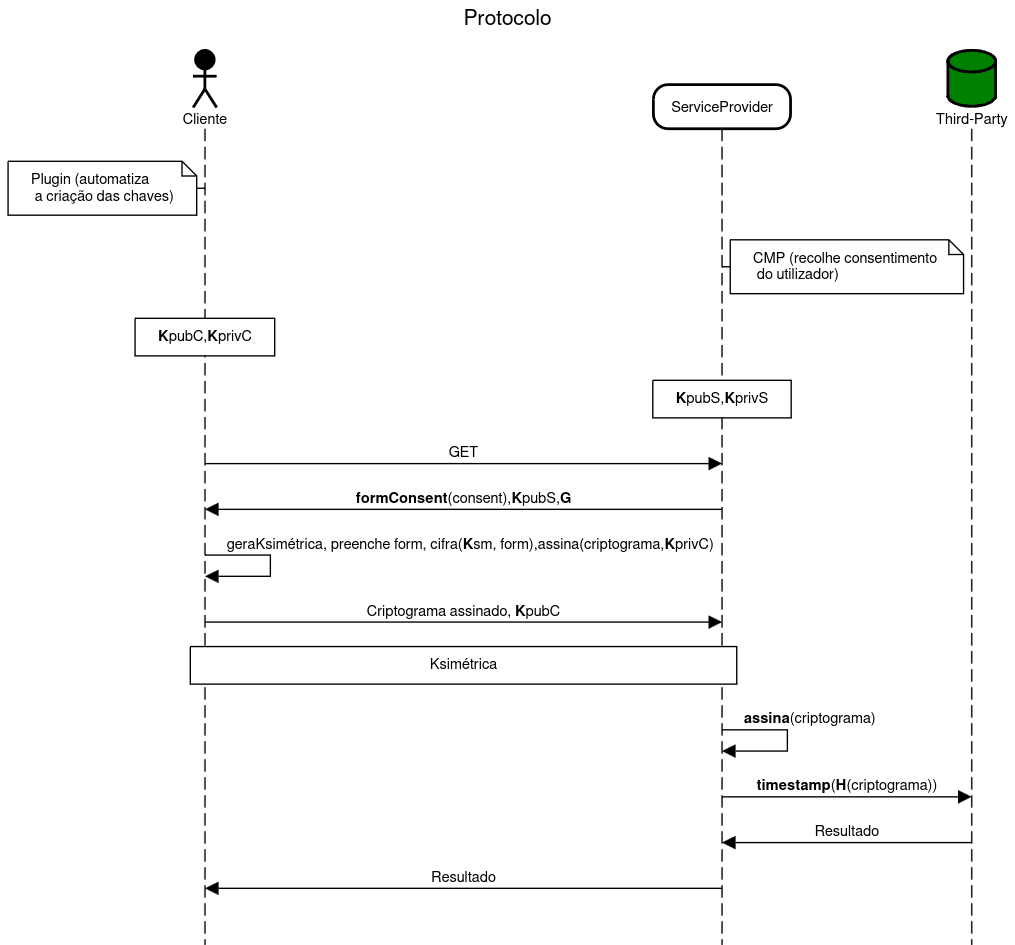
\includegraphics[width=0.8\textwidth]{images/Protocolo.png}
\end{center}
\caption{Diagrama de fluxos da proposta}
\label{fig:esquema}
\end{figure}

\subsection{Lógica de Funcionamento}

A estratégia baseia-se numa abordagem de \textbf{consenso criptográfico bilateral}, onde tanto o cliente como o servidor participam activamente na criação de um registo de consentimento verificável e imutável.

\subsubsection{Princípios Fundamentais}
\begin{itemize}
    \item \textbf{Transparência}: Todos os passos são criptograficamente verificáveis
    \item \textbf{Descentralização}: Nenhuma entidade tem controlo unilateral
    \item \textbf{Não-Repúdio}: Impossibilidade de negar consentimentos dados
    \item \textbf{Auditabilidade}: Histórico completo acessível a ambas as partes
\end{itemize}

\subsection{Algoritmos de criptografia}

A solução utiliza uma estratégia criptográfica baseada em RSA que combina:

\begin{itemize}
    \item \textbf{RSA} para acordo de chaves e cifragem assimétrica
    \item \textbf{AES-GCM} para cifragem simétrica dos dados de consentimento
    \item \textbf{RSA-PSS} para assinaturas digitais bilaterais
    \item \textbf{HKDF} para derivação segura de chaves simétricas
\end{itemize}

\subsection{Protocolo de Consenso}

O protocolo estabelece um acordo criptográfico entre cliente e servidor através de três fases:

\begin{enumerate}
    \item \textbf{Estabelecimento de Confiança}: Troca de chaves públicas RSA
    \item \textbf{Cifragem Segura}: Utilização de RSA para proteger chave simétrica AES
    \item \textbf{Validação Bilateral}: Assinaturas digitais de ambas as partes
\end{enumerate}

\subsection{Lógica de Resolução}

A solução resolve o problema da opacidade através de uma estratégia de \textbf{transparência criptográfica}:

\begin{itemize}
    \item O utilizador possui as chaves necessárias para verificar os seus próprios consentimentos
    \item Todos os registos são matematicamente verificáveis
    \item O processo de consentimento é auditável por ambas as partes
\end{itemize}

Em vez de confiar numa única entidade, a solução distribui a confiança:

\begin{itemize}
    \item \textbf{Cliente}: Controla a cifragem inicial dos dados
    \item \textbf{Servidor}: Valida e co-assina o consentimento  
    \item \textbf{Terceiro Neutro}: Armazena os registos de forma imutável
\end{itemize}

\subsection{Interacção Entre Componentes}

\textbf{Interface Web $\leftrightarrow$ Extensão}

A interface web comunica com a extensão através de eventos DOM:
\begin{itemize}
    \item Detecta acções do utilizador no banner de consentimento
    \item Transmite dados de consentimento para processamento criptográfico
    \item Recebe confirmação de sucesso para feedback ao utilizador
\end{itemize}

\textbf{Extensão $\leftrightarrow$ Servidor}

A extensão estabelece um canal seguro com o servidor:
\begin{itemize}
    \item Obtém chaves públicas RSA do servidor
    \item Envia pacotes de consentimento cifrados e assinados
    \item Recebe validação e assinatura do servidor
\end{itemize}

\textbf{Sistema $\leftrightarrow$ Armazenamento}

Ambos os componentes (extensão e servidor) interagem com o armazenamento:
\begin{itemize}
    \item Enviam registos de consentimento de forma independente
    \item Criam um registo distribuído para auditoria futura
    \item Permitem consulta posterior por ambas as partes
\end{itemize}

\begin{figure}[h]
\begin{center}
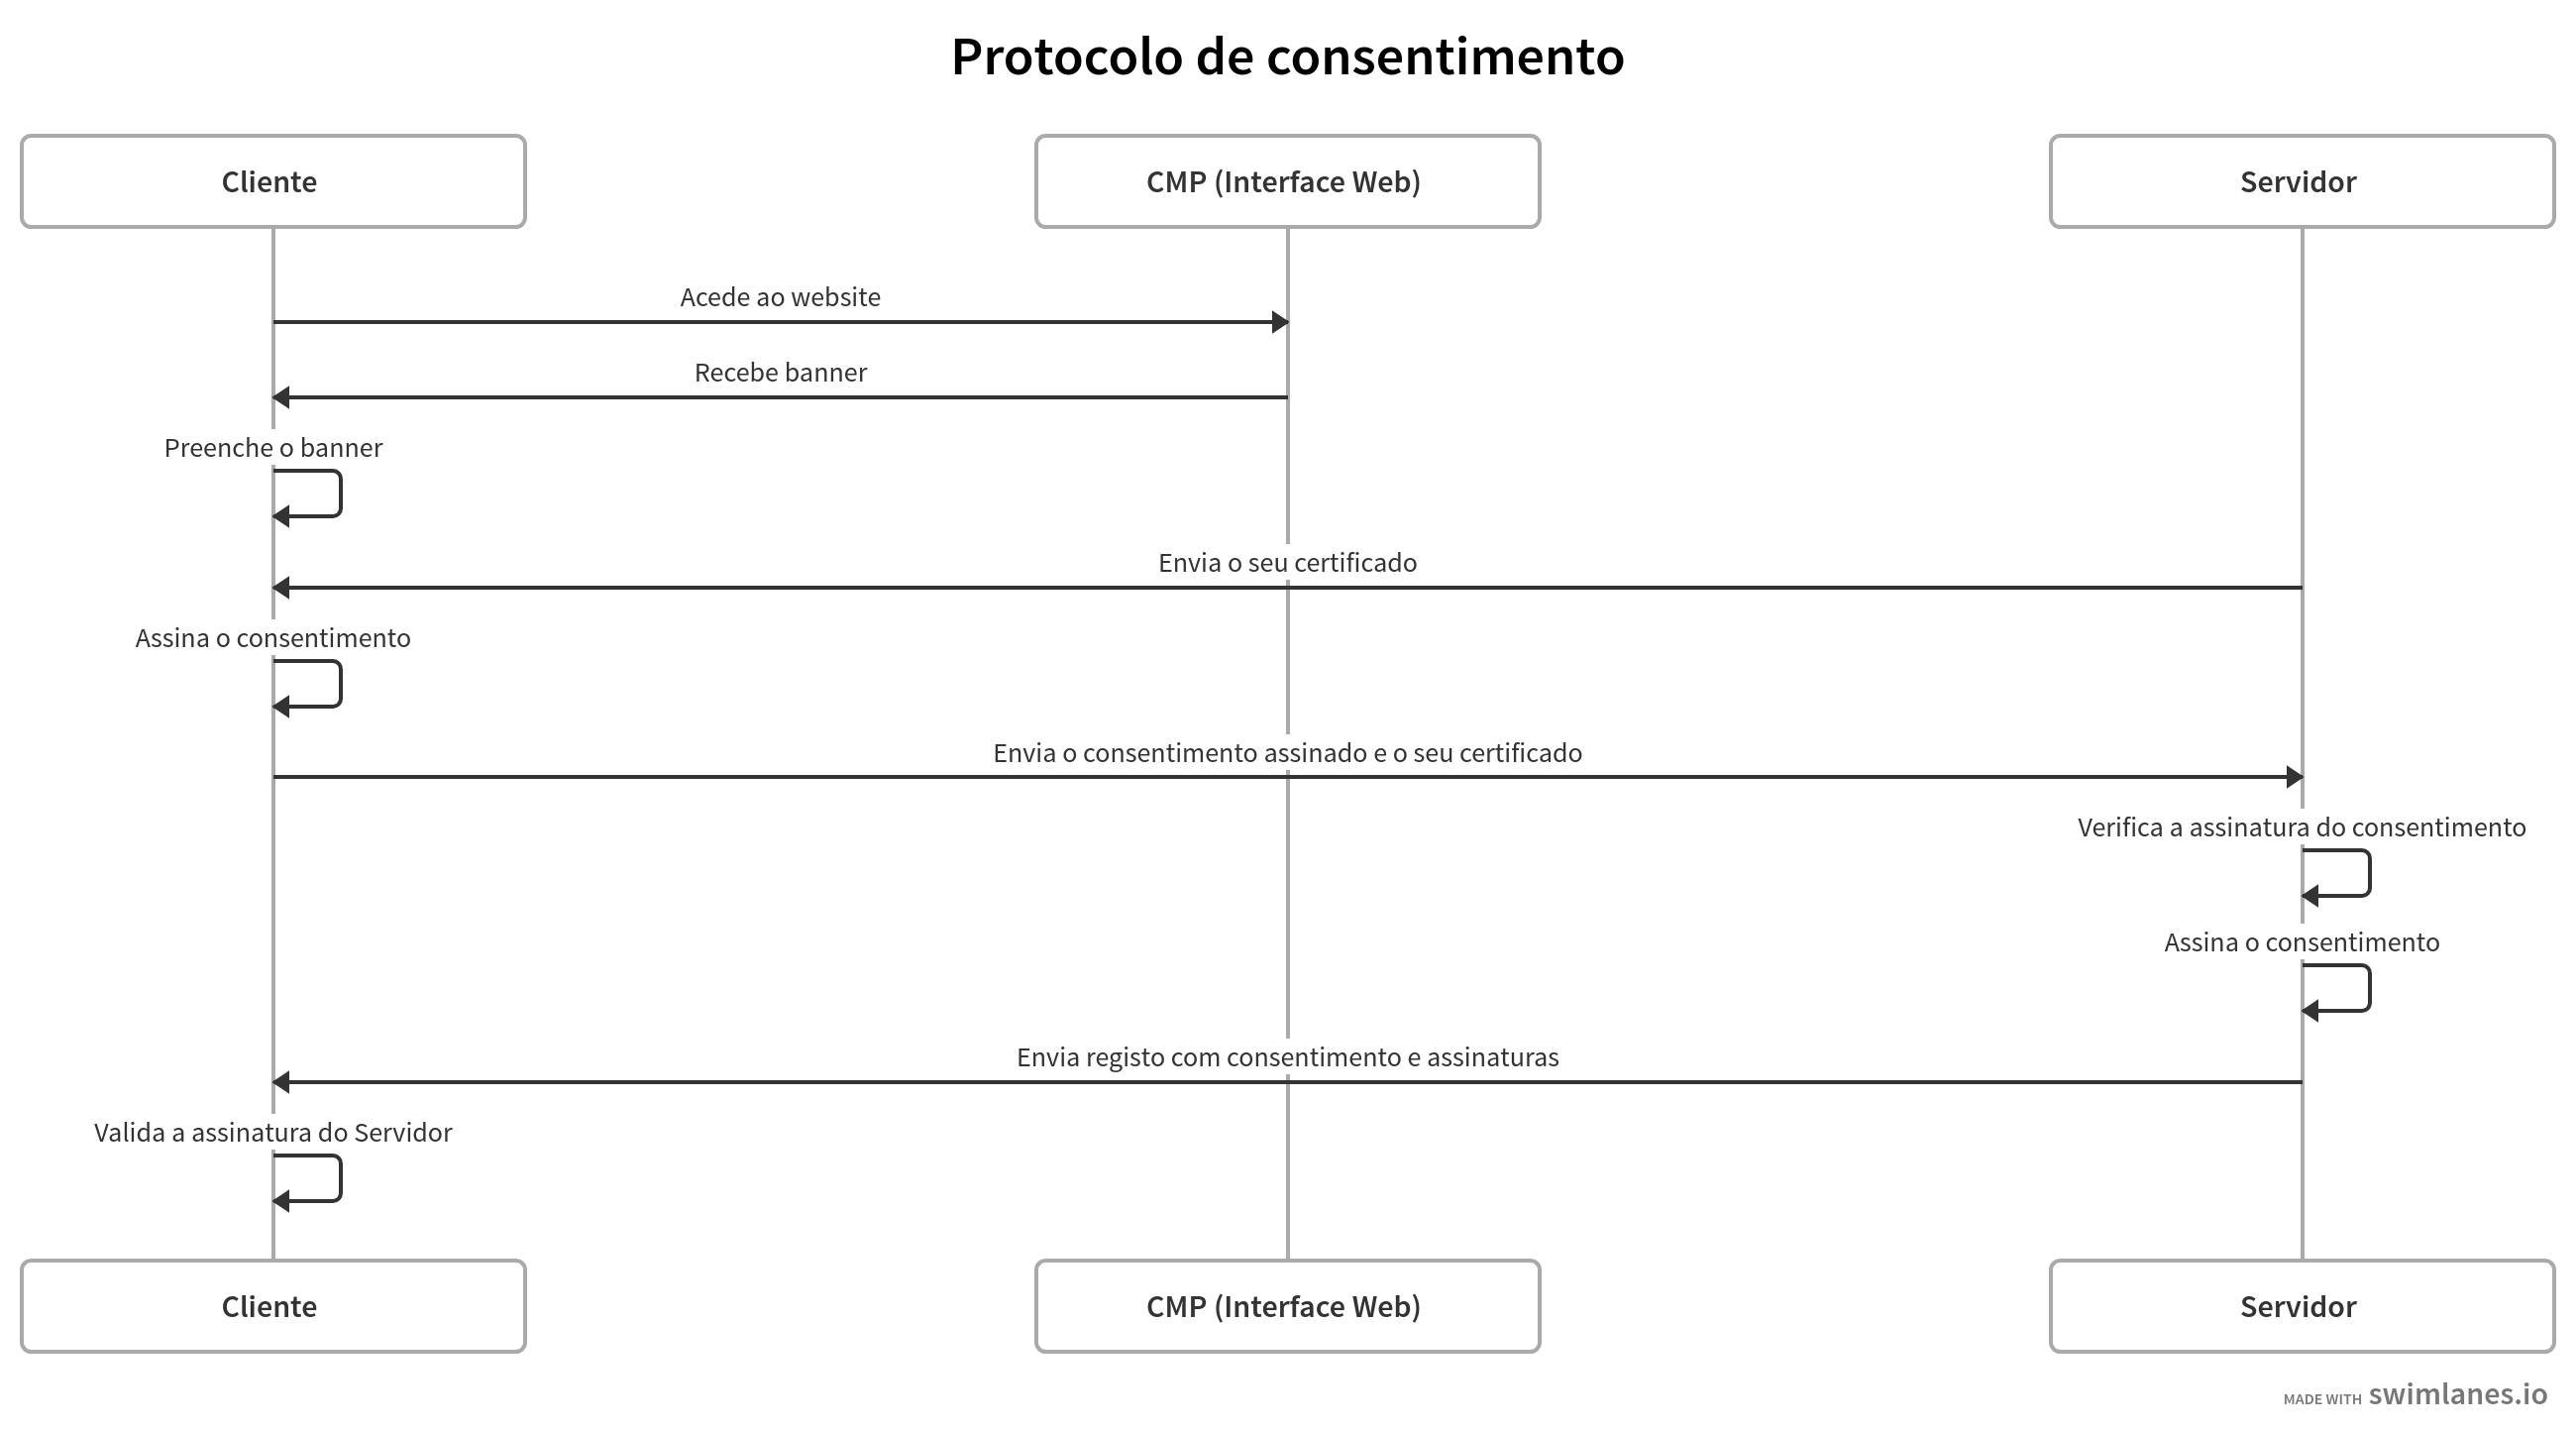
\includegraphics[width=1.0\textwidth]{images/swimlanes.png}
\end{center}
\caption{Diagrama do protocolo}
\label{fig:swimlane}
\end{figure}

\subsection{Benefícios da Arquitectura}

\textbf{Para o Utilizador}
\begin{itemize}
    \item Acesso directo ao histórico de consentimentos
    \item Capacidade de verificar a integridade dos registos
    \item Controlo sobre os próprios dados de consentimento
\end{itemize}

\textbf{Para a Organização}
\begin{itemize}
    \item Prova criptográfica de consentimentos válidos
    \item Redução de riscos de conformidade
    \item Processo de auditoria automatizado
\end{itemize}

\textbf{Arquitecturais}
\begin{itemize}
    \item Escalabilidade através de processamento distribuído
    \item Resistência a falhas por redundância de registos
    \item Interoperabilidade através de protocolos padronizados
\end{itemize}

%\section{Imagens}
%Exemplo de inserção de uma imagem como texto exibido,
%\begin{center}
%	
\includegraphics[width=0.1\textwidth]{images/UM.jpg}
%\end{center}

%\begin{wrapfigure}{r}{0.15\textwidth}	
	%
\includegraphics[width=0.1\textwidth]{images/UM.jpg}
%\end{wrapfigure}
%\noindent --- dentro no texto,
%bla-bla bla-bla bla-bla bla-bla bla-bla bla-bla bla-bla bla-bla bla-bla bla-bla
%bla-bla bla-bla bla-bla bla-bla bla-bla bla-bla bla-bla bla-bla bla-bla bla-bla
%bla-bla bla-bla bla-bla bla-bla bla-bla bla-bla bla-bla bla-bla bla-bla bla-bla
%bla-bla bla-bla bla-bla bla-bla bla-bla bla-bla bla-bla bla-bla bla-bla bla-bla
%bla-bla bla-bla bla-bla bla-bla bla-bla bla-bla bla-bla bla-bla bla-bla bla-bla bla-bla bla-bla bla-bla bla-bla
%bla-bla bla-bla bla-bla bla-bla bla-bla bla-bla bla-bla bla-bla bla-bla bla-bla bla-bla bla-bla bla-bla bla-bla

%\noindent --- ou em formato flutuante
%\begin{figure}
%\begin{center}
%	
\includegraphics[width=0.25\textwidth]{images/UM.jpg}
%\end{center}
%\caption{Legenda}
%\end{figure}
